\documentclass{article}
\usepackage[utf8]{inputenc}

\title{Chem-131C-Lec12}

\author{swflynn }
\date{April 2017}

\usepackage{natbib}
\usepackage{graphicx}
\usepackage{braket}
\usepackage{amsmath}
\usepackage[margin=0.7in]{geometry}
\usepackage{subfigure}
\usepackage{url}

\begin{document}

\maketitle

\section*{Lecture 12; 4/28/17}
Last lecture we began to discuss Maxwell's demon and an apparent violation of the second law.
A demon would place a partition within a box containing 1 molecule, then attaches a piston and do an isothermal expansion into the now evacuated portion of the box.
We can get useful work doing this, violating the second law w = -kTln$\frac{V_f}{V_i}$. 

If you take a gas and then decrease the volume, you decrease the entropy (less volume therefore less conformations available). 
The expansion is done isothermally so q = kTln2 (assume we double the volume). 
The whole cycle has an entropy change of 0, we pull heat from the environment and convert it to useful work. 
$\Delta S_{surr} = \frac{-Q}{T}$ = -kln2.

The key realization (that took 100 years to resolve) is the behavior of the demon. 
People were able to show things like moving the partition and etc would not fix this situation. 
Instead it turns out the Demon must think about what it is doing (it would be incredibly unlikely that the demon could randomly move the partition and always select the correct side to attach the piston). 
Remember, when you complete a cycle the system must return back to its initial configuration. 
It turns out we need to 'reset' our demon, the demon remembers the choice it made and we need to erase that memory.
Be warned, the concept of memory is deeply rooted in dynamics (systems changing in time).
We usually assume, or hope there is no memory in our system (Markovian dynamics), but this is not always true as in the case of the Demon. 

To solve this problem think of the memory as a binomial, the particle can be left or right, 0 or 1. 
So the memory starts with an initial value, but this value may or may not be correct (think in terms of a program, we have initialized the variable but we have not actually set our value). 
The demon must then inspect the system and place the partition accordingly.
It has to record where the particle is to appropriately attach the piston. 
Storing where the particle is in memory costs nothing, attaching the piston costs nothing, the cost comes from resetting the system. 
It turns out that if we are going to perfectly reset the memory, we could imagine taking our binomial and making it a box of its own (the memory is now a particle in a box on either the left or right side). 
If we do the experiment in this way, when we reset the memory we need to remove the partition of the memory.
We then let the particle equilibrate, and finally place the memory partition back in and compress to our initial state. 
In this way it becomes clear that we are going to completely repeat our process, however, we now need to put in the work, and we do exactly as much work as we got out for 'free',  kTln2. 

The moral of the story; there is a connection between theoretical physics, the physical world, and information. 
We are not able to take heat from the environment and do useful work without paying a price (do not trust anyone who says they are violating the laws of thermodynamics).

\subsection*{Heat Engines}
The exam will most probably cover material through Chapter 21. 
Chapter 21 can be summarized as S$\rightarrow$ 0, T$\rightarrow$0. 

With that out of the way let's return to chapter 20 and start discussing engines.

\begin{figure}[! h]
    \centering
    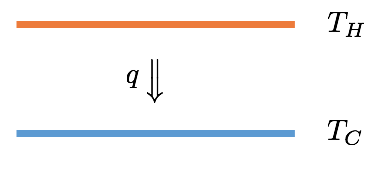
\includegraphics[width=7cm]{thermal.png}
    \caption{'Heat Engine'. Heat is transferred from the higher temperature to the lower temperature spontaneously. No useful work is extracted.}
    \label{fig:thermal}
\end{figure}

A heat engine is essentially just any device where we have a temperature gradient. 
Place the two objects in thermal contact and heat will transfer from the hot material to the cold material. 
This process is spontaneous, we know that the entropy of the universe must increase because we are transferring heat (second law). 
\begin{equation}
\begin{split}
\Delta S_{univ} = \Delta S_{hot} + \Delta S_{cold}\\
\Delta S_{hot}= \frac{-q}{T_h} \qquad \Delta S_{cold} = \frac{q}{t_c} \\
\Delta S_{univ} = \frac{-q}{T_h} + \frac{q}{T_c} = q\left(\frac{1}{T_c} - \frac{1}{T_h} \right) > 0
\end{split}
\end{equation}

To call this an engine would actually be pretty silly, and engineers would remorse.
We had this temperature gradient far from equilibrium ready to do useful work for us, and we just brought the materials into contact and let the heat transfer occur. 
An engineer would want to stick an engine between the two materials and get some useful work out of the system. 
Now the picture looks a little different, we use some of the heat from the hot reservoir to do useful work, and the rest is expelled into the cold reservoir. 
There is no such thing as a perfect engine, we must dump some heat into the cold reservoir.
There is no way to completely convert heat into useful work (nothing is perfectly efficient), and this is how entropy is generally introduced in engineering thermodynamics. 
Ultimately we can't violate the second law, so we will need to dump heat into the cold reservoir to increase the entropy of the universe (think of $q_c$ as your second law tax requirements). 

\begin{figure}[! h]
    \centering
    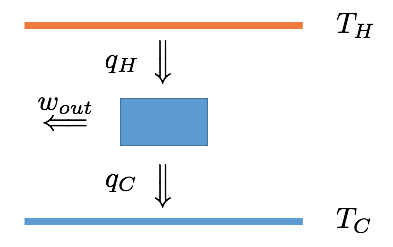
\includegraphics[width=7cm]{heat_engine.png}
    \caption{Heat Engine. Heat is transferred from the higher temperature to the lower temperature spontaneously. Some of the gradient is used to extract work.}
    \label{fig:engine}
\end{figure}

For our engine we would write the first law (we cannot forget about conservation of energy)
\begin{equation}
q_h = w_{out} + q_c
\end{equation} 
Next we can write our second law. 
\begin{equation}
\begin{split}
\Delta S_{univ} \geq 0 = \frac{q_c}{T_c} - \frac{q_h}{T_h}\\
q_c = \frac{T_c}{T_h}q_h
\end{split}
\end{equation}
Where the last line wold be our best possible scenario (the thermodynamic limit). 
This case would coincide with a reversible process, and the total change in entropy would be 0. 
\begin{equation}
w_{out} = q_h - q_c = \left( 1 - \frac{T_c}{T_h}\right)q_h 
\end{equation}
Engineer's like to define the thermodynamic efficiency; $\eta = \left( 1 - \frac{T_c}{T_h}\right)$, and use this as a metric for their systems.  
From looking at the equation we see that the most efficient type of engine would have a very hot material and a very cold material, taking the limits we could get unit efficiency. 

Let's now think about temperature and entropy, as the temperature goes to 0 there is not enough energy for any atoms to leave their ground state, therefore you only have 1 available state in the system and w, S=kln(W) $\rightarrow$ 0. 
You could imagine a type of degeneracy in your ground state $\equiv$ g where maybe the system has 2 equally low energy states at T=0 (imagine a diatomic at different orientation). 
In this case we would find that S=kln(g). 
So remember the entropy can actually be 0, and this is a very well defined property.
Things like energy are arbitrarily set to 0, the total energy of a system cannot be 0, it is the change in energy that we study. 

\subsection*{Adiabatic Irreversible Compression}
If a process is done irreversibly we know that the entropy of the universe is strictly $>$ 0. 
Because the process is adiabatic we know q=0, and subsequently $\Delta S_{surr} = 0$. 
So the first law tells us that $\Delta$U = w. 
When we compress the gas the energy of the gas increases and the final temperature must be larger than the initial temperature. 
To do this is not so trivial, we have 2 unknowns and will then need 2 equations,
We will explore this problem in detail next lecture, the strategy is to substitute equations to solve for the final temperature, and then use this result to substitute in again and solve for final volume. 

\section{Supplemental Information}
I am going to do my best to explain the Maxwell Demon's problem from the stance of a computer. 
I am in no way an expert in this area, however, I do find it very interesting. 
This is going to be a gross oversimplification, hopefully give some intuition to the problem, and to basic computer science.

\subsection{Information}
We can think of the memory in a computer as being 2 distinct things.
One we will call the ram (random access memory), this type of memory is very quickly accesses, and holds information that you are currently working with on the computer. 
The other type of memory a computer has we will call aux (auxiliary memory, the hard drive or a floppy disk), this type of memory is more permanent. 

The two types of memory work in the same manner, you have a collection of switches that can be on or off (0 or 1). 
With one switch you can only encode 2 bits of information, but we know with more switches we can do better (remember a binomial scales as 2$^N$). 
So within both the ram and the aux we just have a collection of switches that are in a sequences of 0 or 1, and we construct a language to give meaning to that sequence. 

\subsection{The Demon}
So let's now consider our demon, and for this example we will consider a system with a bunch of particles, the demon separates the fast moving from slow moving particles to make a gradient, and uses the gradient to get work for free. 

As a particle approaches the partition, she must decide which side of the partition the particle should go, 0 or 1. 
When he makes this decision she does 2 things (insert demon gender here), he marks it down in both the aux at position a, and then marks it in the ram at position x. 
Once he makes this choice he must remember it until all of the particle in our system have been sorted (remember the particles will randomly bump into the partition he needs to know if he already counted that particle or not). 
If he now wants to repeat the process again (another particle approaches the partition), he will do things slightly different.
When particle 2 comes along he will again make a choice, which side of the box will it go. 
He will record his choice in aux at position b now, but to save space he will record this result in position x again in ram. 
So this is why we have 2 different forms, this is going to be a long calculation, there are alot of particles, he needs to make quick choices about each particle (ram) but does not want to mess up and have to double check his work (aux).
The demon can keep recording this information very easily, at no cost.... until he starts to run out of space.
So when a single particle approaches the partition there is no cost, the demon can open or close it without a problem.
The cost comes when the aux memory needs to be reset.

Remember, we are considering the entropy of the entire cycle, each time a particle moves is just one step in the cycle, we need to complete the whole cycle. 
For the demon to complete the cycle, its memory must return to its original state. 
If the demon simply erased the current value in ram we are NOT at the beginning of our cycle.
The demon must go and physically erase all of the information stored in the aux too. 
To do this the demon needs to run over to aux and randomly flip all the switches (like shuffling a deck of cards).
This is where the thought experiment breaks down, to finish the cycle we must clear both types of memory, and this is what takes energy!

This is similar to how your computer works, there are actually 3 different ways to 'delete' a file. 
Remember your computer is a physical thing, when you store information you physically change the physical material of the computer. 
The switches are a bunch of ferromagnetic molecules pointing in different directions, and their orientation is what encodes the information on your computer. 
The first way to delete (quick delete) just tells your computer the location in memory can be overwritten.
This does not change the orientation of the atoms you used to write this first bit of information, it just moves to a new location and changes a different set of molecules, and uses their result to write to ram. 
So when you just simply delete a file it is very likely someone could go on your computer and find that original information, it has not been removed you simply aren't looking at it anymore. 
So the cost comes from actually deleting the information, this is done by taking all those ferromagnetic atoms you changed around and resetting them.
To reset them you need to put them back into a random orientation. 
One way to picture this would be to excite the atoms (put in heat) and then let them all relax back down to ground state (this will be done randomly).
When they relax back down we know the energy that went  in to exciting them must be dissipated to the environment, generating entropy. 
This heat will necessarily be related to how much information you need to erase, an idea called \textbf{Landauer's Principle}.
This process must be irreversible (that is the whole point we need to get a random orientation again). 
And the minimum energy to erase a bit theoretically has been calculated to be ln(2). 

This is just how I think about this process, do not worry if it makes no sense (I may have just confused you more). 
If you are interested in these types of ideas (remember computers run the world around you) the best place to start besides Google and Wikipedia would be 'The Thermodynamics of Computation, a Review' by Bennett. 

\end{document}